
\documentclass[12pt]{article}

% including packages
\usepackage[utf8]{inputenc}
\usepackage[english]{babel}
\usepackage{amsmath}
\usepackage{graphicx}
\usepackage{wrapfig}
\usepackage[a4paper, total={6in, 8in}]{geometry}
\usepackage{hyperref}
\usepackage{hypcap}
\usepackage[autostyle]{csquotes}
\usepackage[]{biblatex}
\usepackage{amsfonts}

% preferences
\graphicspath{ {images/} }
\newcommand{\lineSeparationLength}{2mm}
\hypersetup{colorlinks=true, allcolors=black}
\addbibresource{references.bib}
\ExecuteBibliographyOptions{
	giveninits=true,
	isbn=false,
	doi=false,
	url=false
}
\setlength{\parskip}{1em}
\newcommand{\textem}[1]{\textbf{\textit{#1}}}

% title
\title{Using Genetic Algorithms to Find Approximations for the Minimum Vertex Cover Problem}
\author{}
\date{}





% document begins here
\begin{document}

% cover page
\pagenumbering{roman}
\cleardoublepage\phantomsection\addcontentsline{toc}{section}{Cover Page}

{
\begin{wrapfigure}{r}{0.25\textwidth}
\hfill
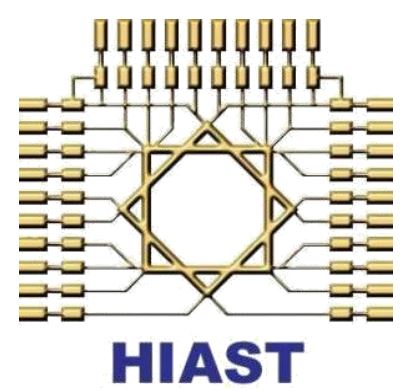
\includegraphics[width=0.9\linewidth]{hiast}
\end{wrapfigure}

\ \\[\lineSeparationLength]
Syrian Arab Republic \\[\lineSeparationLength]
Higher Institute for Applied Sciences and Technology \\[\lineSeparationLength]
Informatics Department \\[\lineSeparationLength]
Fourth Year
}

\vspace{25mm}
{\let\newpage\relax\maketitle}

\vspace{-10mm}
\begin{center}
Keywords: genetic algorithms, NP-complete, combinatorial optimization, non-deterministic algorithms, approximation algorithms, minimum vertex cover.
\end{center}

\vspace{5mm}
\begin{center}
\begin{align*}
\text{Author: }					& \textit{Farouk Hjabo} \\
\text{Academic Supervisor: }	& \textit{Dr. Said Desouki} \\
\text{General Supervisor: }		& \textit{Dr. Kadan Aljoumaa} \\
\text{Langauge Supervisor: }	& \textit{Mr. Fahmi Alammareen} \\
\end{align*}
\end{center}

\vfill
\centerline{\date{\today}}
\thispagestyle{empty}
\pagebreak

% abstract page
\cleardoublepage\phantomsection\addcontentsline{toc}{section}{Abstract}

\begin{abstract}
Lorem ipsum dolor sit amet, consectetur adipisicing elit, sed do eiusmod
tempor incididunt ut labore et dolore magna aliqua. Ut enim ad minim veniam,
quis nostrud exercitation ullamco laboris nisi ut aliquip ex ea commodo
consequat. Duis aute irure dolor in reprehenderit in voluptate velit esse
cillum dolore eu fugiat nulla pariatur. Excepteur sint occaecat cupidatat non
proident, sunt in culpa qui officia deserunt mollit anim id est laborum.
\end{abstract}

\vfill

\noindent
\textit{
``It is not the strongest of the species that survives,
nor the most intelligent, but the one most responsive
to change.''
}
\begin{flushright}
\setlength{\parskip}{0em}
\rm --- Charles Darwin
\end{flushright}

\pagebreak


% table of contents page
\cleardoublepage\phantomsection\addcontentsline{toc}{section}{Contents}
\tableofcontents
\pagebreak




% first page starts here
\pagenumbering{arabic}

\section{Introduction}
Once the NP-hardness of a combinatorial optimization
problem is established, the search for an optimal solution
is abandoned. The goal then becomes one of finding a
good heuristic, i.e. a polynomial running time algorithm
that can find solutions close to the optimal. In most cases,
traditional heuristics are problem dependent; a heuristic is
tailored to the specific problem it is trying to solve.

In this paper, we present an alternative approach that
uses genetic algorithms as a generalized heuristic for solving NP-hard combinatorial optimization problems. The
application of a genetic algorithm is demonstrated here for
the \emph{minimum vertex cover} problem. These algorithms
have been successfully applied to a broad range of problems. This wide range can be tackled by genetic algorithms
mainly due to the fact that they work with an encoding of
the domain rather than with the problem domain itself.


\section{Genetic Algorithms}
\subsection{The Intuition Behind GAs}
Genetic Algorithms (GAs)~\cite{goldberg1989genetic} are population based
search algorithms, where by repeated use of genetic operations,
such as \textem{mutation}, \textem{selection}, \textem{crossover}, etc...
Successive new generations of better populations in the direction of
search objectives are created. They are inspired by Darwinian principles
based on natural evolution. In other words, the main idea behind genetic
algorithms is that only the \textem{fittest} individuals will survive.\\
Main advantage of genetic algorithms is that they ideally do not make
any assumption about the underlying problem, hence they are suitable to tackle
a wide range of diverse problems in
engineering, art, biology, economics, marketing, genetics,
operations research, robotics, social sciences, physics, politics, chemistry,
etc...

\noindent
So what is a GA? A typical GA consists of the following:
\vspace{-5mm}
\begin{enumerate}
\setlength{\parskip}{0em}
\item a number, or \textem{population}, of candidate solutions to the problem.
\item a way of calculating how good or bad the individual solutions within the
population are. i.e. how \textem{fit} an individual is?
\item a method for mixing fragments of the better solutions to form new, on
average even better solutions. Which permits the population to \textem{evolve} naturally.
\item a \textem{mutation} operator to avoid permanent loss of diversity within the
solutions. This allows introducing new information in the population.
\end{enumerate}

\subsection{Typical GA Schema}
The basic iteration cycle of a genetic algorithm proceeds on a population
of individuals, each of which represents a search point in the space
of potential solutions of a given optimization problem.
In case of a canonical genetic algorithm, each individual is a binary vector
$ \vec{x} = ( x_1, x_2, \dots, x_n ) \in \{0, 1\}^n $
of fixed length $n$. The fitness function
$ f: \{0, 1\}^n \rightarrow \mathbb{R} $
provides a quality measure which is used by the selection procedure to direct
the search towards regions of the search space where the
average fitness of the population increases. The recombination operator
allows for the exchange of information between different individuals, and
mutation introduces innovation into the population.

After a uniform random initialization of the population
the evolution proceeds by iterating the steps selection,
recombination (crossover), and mutation (see figure~\ref{fig:ga})
until a termination criterion is fulfilled.
In most cases, the algorithm is terminated after a certain number of
iterations of the basic cycle or when a satisfactory fitness
level has been reached.

The recombination (crossover) operator allows for the
exchange of information between different individuals. The
original one-point crossover [9] works on two parent individuals
(which are randomly chosen from the population, see the next paragraph)
by choosing a crossover point $ \chi \in \{1, \dots, n-1 \} $
at random and exchanging all bits after the $ \chi^{\text{th}} $ one
between both individuals. The crossover rate
$ p_c \ (\text{e.g. } p_c \approx 0.6) $
determines the probability to undergo crossover (see todo for more details).
The crossover operator can be extended to a generalized
multi-point crossover [10] or even to uniform crossover,
where an it is randomly decided for each bit
whether to exchange it or not [19]. The strong mixing effect
introduced by uniform crossover is sometimes helpful
to overcome local optima.

Normally, selection in genetic algorithms is a probabilistic operator
which uses the relative fitness 
$ p_s \left( \vec{x_i} \right) = 
f \left( \vec{x_i} \right) / \sum_{j=1}^uf \left( \vec{x_j} \right) $
to serve as selection probabilities
($u$ denotes the population size). This selection operator
is called proportional selection. If the problem under
consideration is a minimization one, or if the fitness
function can take negative values, then $ f \left( \vec{x_i} \right) $ has to be
linearly transformed before calculating selection probabilities.
This technique known as linear dynamic scaling is commonly used
in genetic algorithms (see [13], pp. 123-124, or [14]).

Innovation, i.e. new information, is introduced into the
population by means of mutation, which works by inverting
bits with a small probability
$ p_m \ (\text{e.g. } p_m \approx 0.001) $
Though mutation is often interpreted as a rather unimportant operator
in genetic algorithms [9], recent theoretical
work gives strong evidence for an appropriate choice of a
mutation rate $ p_m = 1/n $ on many problems [2; 12].


\begin{figure}[ht]
\centering
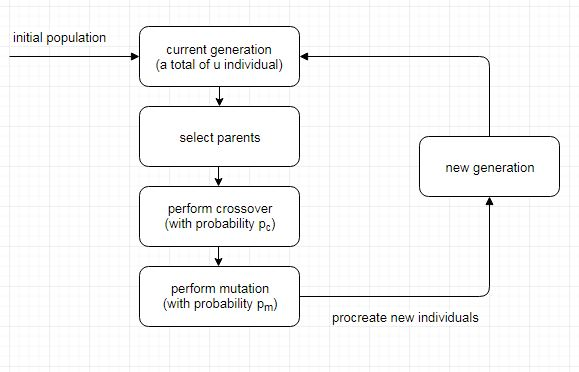
\includegraphics[width=1\textwidth]{ga}
\caption{general schema for genetic algorithms}
\label{fig:ga}
\end{figure}



\section{The Minimum Vertex Cover Problem}
Lorem \cite{einstein} ipsum dolor sit amet, consectetur adipisicing elit, sed do eiusmod
tempor incididunt ut labore et dolore magna aliqua. Ut enim ad minim veniam,
quis nostrud exercitation ullamco laboris nisi ut aliquip ex ea commodo
consequat. Duis aute irure dolor in reprehenderit in voluptate velit esse
cillum dolore eu fugiat nulla pariatur. Excepteur sint occaecat cupidatat non
proident, sunt in culpa qui officia deserunt mollit anim id est laborum.


\section{Experimental Results}
Lorem \cite{dirac} ipsum dolor sit amet, consectetur adipisicing elit, sed do eiusmod
tempor incididunt ut labore et dolore magna aliqua. Ut enim ad minim veniam,
quis nostrud exercitation ullamco laboris nisi ut aliquip ex ea commodo
consequat. Duis aute irure dolor in reprehenderit in voluptate velit esse
cillum dolore eu fugiat nulla pariatur. Excepteur sint occaecat cupidatat non
proident, sunt in culpa qui officia deserunt mollit anim id est laborum.


\section{Conclusion}
sit amet, consectetur adipisicing elit, sed do eiusmod


\pagebreak


\cleardoublepage\phantomsection\addcontentsline{toc}{section}{References}
%\bibliographystyle{abbrv}
%\bibliography{references}
\printbibliography

% end of document
\end{document}


